\section{Scheduled Event List}
\label{sec:theory-sel}

Once the warehouse operations have been represented as discrete events, it is
necessary to determine how these events evolve during the simulation. A useful
technique for this purpose is the \textit{Scheduled Event List} (SEL), which
provides a mechanism for managing the events that may occur as the state of the
system changes, following the discrete-event simulation framework described
in~\cite{cassandras2021des}.

The basic idea is to associate each feasible event with the instant of time at
which it is expected to occur. Considering a set of events $E$ and a state space
$X$, at a given state $x \in X$ only a subset of events is feasible. This subset
can be denoted by $\Gamma(x)$. Each feasible event $i \in \Gamma(x)$ is associated
with a clock value $y_i$, representing the amount of time remaining before that
event occurs.

The next event to be executed is therefore the feasible event characterized by
the smallest clock value:

\begin{equation}
	e' = \arg\min_{i \in \Gamma(x)} y_i
\end{equation}


\noindent Consequently, the amount of time spent in the current state is

\begin{equation}
	y^* = \min_{i \in \Gamma(x)} y_i
\end{equation}

\noindent and the simulation time can be updated according to

\begin{equation}
	t' = t + y^*
\end{equation}

\noindent Instead of explicitly maintaining the remaining clock value of every event, the
simulation can store the events together with their scheduled execution times.
The resulting Scheduled Event List can be represented as

\[
L = \{(e_k,t_k)\},
\]

\noindent where $e_k$ represents an event and $t_k$ the corresponding scheduled execution
time.

The evolution of the simulation can then be described as an iterative procedure.
First, the event having the smallest scheduled time is extracted from the SEL
and executed. The simulation clock is advanced to the corresponding event time
and the state of the system is updated. As a consequence of this state change,
some previously scheduled events may no longer be feasible and are therefore
removed from the list, while newly enabled events are inserted. Finally, the SEL
is reordered according to the scheduled execution times before starting the next
iteration.

\begin{figure}[H]
	\centering
	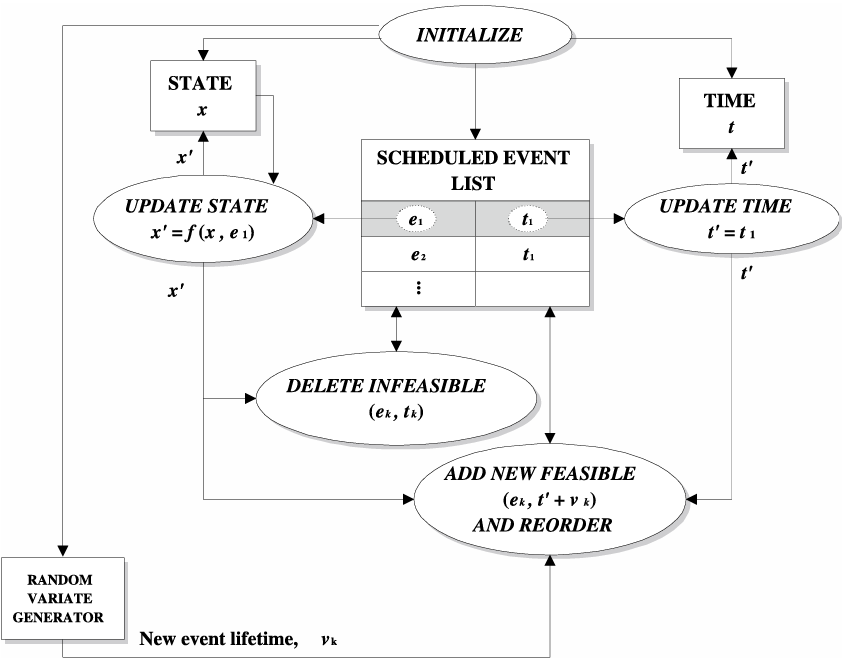
\includegraphics[width=1\linewidth]{imgs/Cap2_teoria/SEL_generalized}
	\caption{Generalized Scheduling Event scheme in computer simulations}
	\label{fig:selgeneralized}
\end{figure}


In the warehouse scheduling problem, this mechanism is particularly useful
because the feasibility of a mission depends on the current state and on the
availability of the resources required to execute it. For example, a loading
operation requiring both a forklift and an operator cannot start until both
resources are available. When another mission is completed and those resources
are released, the state of the system changes and the loading operation may
become feasible and consequently enter the SEL.

The SEL should therefore not be interpreted as a static schedule generated once
at the beginning of the simulation. It is a dynamic structure that evolves
together with the system. This is particularly important when several missions
compete for shared resources, since every completed operation may modify the set
of missions that can subsequently be executed.

In this framework, the SEL provides the temporal mechanism required to determine
\textit{when} events occur. However, an additional model is required to represent
the state of the system, the availability of resources, the dependencies between
operations, and the conditions under which an event becomes feasible. In the
proposed design, admission to a resource queue is an additional scheduling
condition: an enabled operation must also have been admitted before it can
start. Queue replenishment determines which missions enter execution, whereas
the event mechanism orders their simulated state changes. Petri nets
provide a suitable formalism for this purpose.


\section{Petri Nets}

Warehouse operations are characterized by a high degree of concurrency. Several
missions may be active at the same time, different resources may operate
simultaneously, and multiple activities may compete for the same limited
resources. A model used to represent such a system must therefore describe not
only the individual evolution of each mission, but also synchronization,
concurrency, resource availability, and conflicts among different activities.

\textit{Petri nets} (PNs) are a discrete-event modeling formalism particularly
suited to representing these characteristics. A Petri net is a directed bipartite
graph composed of two different types of nodes: \textit{places} and
\textit{transitions}. Places can represent conditions, states, or the availability
of resources, whereas transitions represent events or operations that modify the
state of the system. Places and transitions are connected through directed arcs.
The terminology and firing rules used here follow the formulation
in~\cite{murata1989petri,cassandras2021des}; the use of Petri-net models
for simulation and control is also discussed
in~\cite{basile2007pnetlab}.

The current state of a Petri net is described by its \textit{marking}, namely the
distribution of \textit{tokens} among the places of the net. A transition is
enabled only when its input places contain the tokens required for its execution.
When an enabled transition fires, the corresponding input tokens are consumed
and new tokens are produced in its output places, according to the structure of
the net.

This mechanism naturally represents resource allocation. For example, consider
a warehouse mission that requires both a forklift and an operator. Two places
may represent the availability of these resources. The transition corresponding
to the beginning of the mission can fire only when both places contain the
required tokens. Once the transition fires, the tokens are removed, representing
the fact that the forklift and the operator are currently busy. At the completion
of the mission, another transition can return the tokens to the corresponding
resource-availability places, making them available for subsequent missions.

This representation becomes particularly useful when several missions compete
for the same resources. If two missions require the same forklift, for example,
the availability of a single token prevents both corresponding transitions from
acquiring that resource simultaneously (fig. \ref{fig:pn}). Resource conflicts can therefore be
represented directly through the structure and marking of the net.

\begin{figure}[H]
	\centering
	
	\begin{subfigure}[b]{0.48\textwidth}
		\centering
		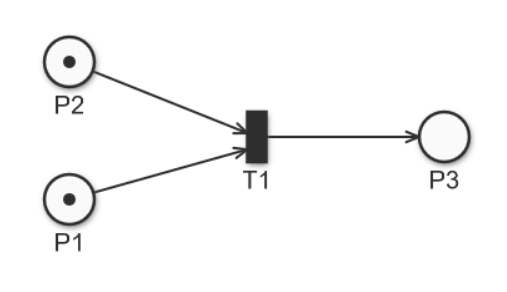
\includegraphics[width=\textwidth]{imgs/Cap2_teoria/pn1.png}
		\caption{Before triggering $t1$}
		\label{fig:pn1}
	\end{subfigure}
	\hfill
	\begin{subfigure}[b]{0.48\textwidth}
		\centering
		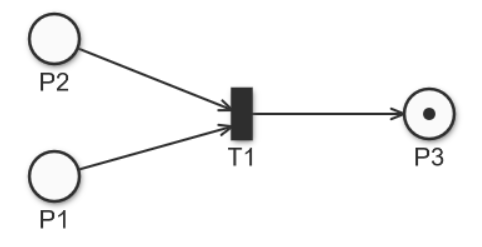
\includegraphics[width=\textwidth]{imgs/Cap2_teoria/pn2.png}
		\caption{After triggering $t1$}
		\label{fig:pn2}
	\end{subfigure}
	
	\caption{Example of petri net transition firing}
	\label{fig:pn}
\end{figure}

\noindent Compared with a representation based exclusively on finite-state machines,
Petri nets provide a natural way to describe several concurrent activities within
the same model. This characteristic is especially relevant in warehouse systems,
where many missions may evolve simultaneously and their execution may depend on
shared resources.

Petri nets can also be represented mathematically through incidence
matrices~\cite{murata1989petri}.
In particular, the \textit{Pre} and \textit{Post} matrices describe the
connections from places to transitions and from transitions to places,
respectively. This representation is particularly useful when the model has to be
automatically generated, simulated, or integrated into an optimization algorithm.

From a mathematical point of view, a Place/Transition Petri Net can be defined
as the four-tuple $N = (P,T,Pre,Post)$ where $P$ is the set of places, $T$ is the set of transitions, while $Pre$ and $Post$ describe the connections between places and transitions.

The structure of the net can also be represented through the incidence matrix

\begin{equation}
	C = Post - Pre
\end{equation}

\noindent The state of the system is represented by the \textit{marking} $m$, which
specifies the number of tokens contained in each place. A transition $t$ is
enabled only if all its input places contain the required number of tokens:

\begin{equation}
	m(p) \geq Pre(p,t),
	\qquad \forall p \in {}^\bullet t
\end{equation}

\noindent When an enabled transition fires, the marking of the Petri Net changes according
to the tokens consumed and produced by the transition. More generally, the
evolution of the marking after a sequence of transition firings can be expressed
through the state equation

\begin{equation}
	m = m_0 + C\sigma
\end{equation}

\noindent where $m_0$ is the initial marking and $\sigma$ is the firing-count vector,
whose elements indicate how many times each transition has fired.

\subsection{Colored Petri Nets}

When the system contains a large number of missions and several similar resources,
a standard Petri-net representation may become increasingly complex. A useful
extension is represented by \textit{Colored Petri Nets} (CPNs), which introduce
different types of tokens, generally referred to as \textit{colors}. The basic
concepts and modeling principles of CPNs are presented
in~\cite{jensen1997coloured}, while their use for discrete-event simulation
and control is discussed in~\cite{basile2007pnetlab}.

The use of colors makes it possible to distinguish different resources or
operational conditions while preserving the general structure of the Petri net.
In a warehouse scenario, for example, different colors can be associated with
different operators and forklifts combination involved in mission execution.
In this way, multiple resources can evolve simultaneously through the same model
without losing information about which specific resource is performing a given
task.

Formally, a Colored Petri Net can be defined as the six-tuple

\[
N=(P,T,Pre,Post,Cl,Co),
\]

\noindent where $P$ is the set of places, $T$ is the set of transitions, $Cl$ is the set
of colors, and $Co : P \cup T \rightarrow 2^{Cl}$ is the color function that associates each place and transition with an ordered
set of admissible colors.

For a place $p_i \in P$, the set of possible token colors can be expressed as

\begin{equation}
	Co(p_i)=\{a_{i,1},a_{i,2},\dots,a_{i,u_i}\}\subseteq Cl,
\end{equation}

\noindent while, for a transition $t_j \in T$, the corresponding set of occurrence
colors is

\begin{equation}
	Co(t_j)=\{b_{j,1},b_{j,2},\dots,b_{j,v_j}\}\subseteq Cl.
\end{equation}

\noindent Unlike a standard Petri Net, in which the marking of a place is represented only
by the total number of tokens, in a CPN the marking must also preserve information
about their colors. Therefore, the marking of a place $p_i$ can be represented
by the vector

\[
m_i =
\begin{bmatrix}
	m_i(1)\\
	m_i(2)\\
	\vdots\\
	m_i(u_i)
\end{bmatrix},
\]

\noindent where $m_i(h)$ represents the number of tokens of color $a_{i,h}$ contained in
place $p_i$. The complete marking of the CPN is consequently obtained by
collecting the markings of all places:

\[
m =
\begin{bmatrix}
	m_1\\
	m_2\\
	\vdots\\
	m_{|P|}
\end{bmatrix}.
\]

\noindent This additional information is particularly useful for warehouse optimization.
For example, if several operators are available, each operator can be associated
with a different token color. When a transition corresponding to a mission fires,
the color involved in that transition identifies the particular resource assigned
to the mission.

As in standard Petri Nets, the structural evolution of the system is described
through the incidence matrix

\[
C = Post - Pre.
\]

\noindent However, in a CPN the entries of the $Pre$ and $Post$ matrices also depend on the colors associated with places and transitions.

Considering a transition $t_j$ with occurrence color $b_{j,k}$, the transition
is enabled only if the required number of tokens of each color is available in
its input places:

\begin{equation}
	m_i(h) \geq Pre(p_i,t_j)(h,k).
\end{equation}

\noindent If the transition fires, the marking is updated according to

\begin{equation}
	m_i'(h)
	=
	m_i(h)
	+
	Post(p_i,t_j)(h,k)
	-
	Pre(p_i,t_j)(h,k).
\end{equation}

\noindent These equations show why the introduction of colors is particularly useful in a
resource-allocation problem. The enabling of a transition does not depend only
on the total availability of resources, but also on the availability of the
specific type or identity of resource required by that operation.

For instance, if a mission requires a particular combination operator/forklift, the corresponding transition can be enabled only when the appropriate
token is present in the required places. Once the transition fires, those
token is consumed or moved, representing the fact that the corresponding
resource is currently allocated to the mission. When the operation is completed,
the resource can be released and become available again for other missions.

As a consequence, Colored Petri Nets allow the simulation to keep track of the
usage and identity of individual resources while maintaining the main advantages
of standard Petri Nets in representing concurrency, synchronization, and resource
conflicts. This makes them particularly suitable for resource-allocation and
scheduling problems involving a large number of simultaneous warehouse operations.

\subsubsection{Transition firing example}

In Figure \ref{fig:cpn}, transition $T_1$ has two input places, $P_1$ and $P_2$, containing one blue token and one red token, respectively. Since both input tokens are required, $T_1$ can fire only when they are simultaneously available.

Assuming the color order
\[
[\text{blue},\text{red}],
\]
the token-color vector associated with the firing of $T_1$ is

\[
\mathbf{c}_{T_1}=
\begin{bmatrix}
	1\\
	1
\end{bmatrix}.
\]

\noindent Since $T_1$ preserves the token colors, its color transformation matrix is

\[
\mathbf{A}_{T_1}=
\begin{bmatrix}
	1 & 0\\
	0 & 1
\end{bmatrix}.
\]

\noindent Therefore,

\[
\mathbf{A}_{T_1}\mathbf{c}_{T_1}
=
\begin{bmatrix}
	1\\
	1
\end{bmatrix},
\]

\noindent meaning that one blue token and one red token are simultaneously produced in $P_3$ after the firing.

\begin{figure}[H]
	\centering
	
	\begin{subfigure}[b]{0.48\textwidth}
		\centering
		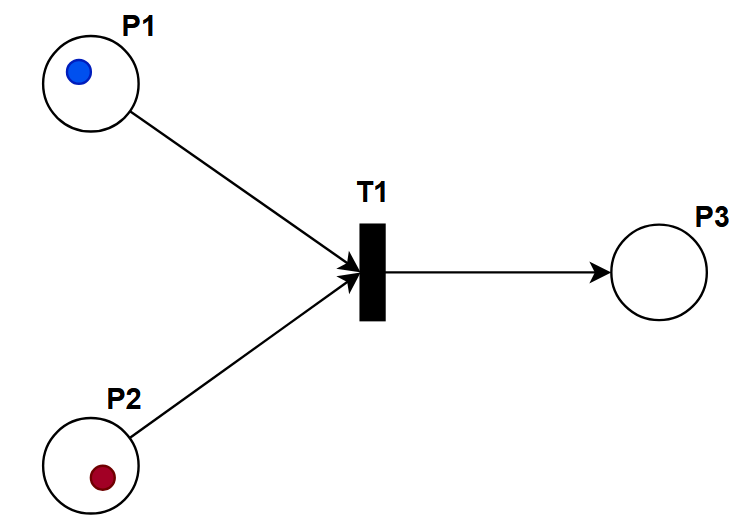
\includegraphics[width=\textwidth]{imgs/Cap2_teoria/CPN1.png}
		\caption{Before firing $T_1$}
		\label{fig:cpn1}
	\end{subfigure}
	\hfill
	\begin{subfigure}[b]{0.48\textwidth}
		\centering
		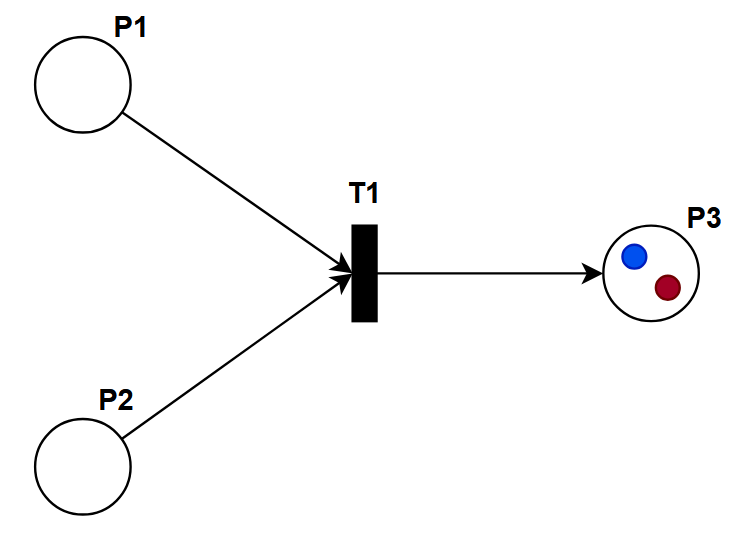
\includegraphics[width=\textwidth]{imgs/Cap2_teoria/CPN3.png}
		\caption{After firing $T_1$}
		\label{fig:cpn2}
	\end{subfigure}
	
	\caption{Example of transition firing in a Colored Petri Net.}
	\label{fig:cpn}
\end{figure}

\noindent Initially, the colored markings of the individual places are

\[
M_0(P_1)=
\begin{bmatrix}
	1 & 0
\end{bmatrix}^{\mathsf T},
\qquad
M_0(P_2)=
\begin{bmatrix}
	0 & 1
\end{bmatrix}^{\mathsf T},
\qquad
M_0(P_3)=
\begin{bmatrix}
	0 & 0
\end{bmatrix}^{\mathsf T}.
\]

\noindent Considering the component order

\[
(P_1^{b},P_1^{r},
P_2^{b},P_2^{r},
P_3^{b},P_3^{r}),
\]

\noindent the global colored marking can equivalently be written as

\[
M_0=
\begin{bmatrix}
	1 & 0 & 0 & 1 & 0 & 0
\end{bmatrix}^{\mathsf T}.
\]

\noindent Since transition $T_1$ consumes one blue token from $P_1$ and one red token from $P_2$, while producing both tokens in $P_3$, the corresponding colored incidence vector is

\[
C_{T_1}
=
\begin{bmatrix}
	-1 & 0 & 0 & -1 & 1 & 1
\end{bmatrix}^{\mathsf T}.
\]

\noindent The new marking after the firing of $T_1$ is obtained through the marking equation

\[
M_1=M_0+C_{T_1},
\]

\noindent hence

\[
M_1=
\begin{bmatrix}
	1\\
	0\\
	0\\
	1\\
	0\\
	0
\end{bmatrix}
+
\begin{bmatrix}
	-1\\
	0\\
	0\\
	-1\\
	1\\
	1
\end{bmatrix}
=
\begin{bmatrix}
	0\\
	0\\
	0\\
	0\\
	1\\
	1
\end{bmatrix}.
\]

\noindent Therefore, after the firing of $T_1$, both input places are empty, while $P_3$ contains one blue token and one red token.

\subsection{Colored Timed Petri Nets and persistent state}
\label{sec:theory-ctpn}

A Colored Timed Petri Net (CTPN) adds timing information to the colored
state representation. In the warehouse model, a mission that starts at
$s_m$ and has simulated duration $\tau_m$ completes at $c_m=s_m+\tau_m$.
The marking and token colors encode precedence and resource ownership,
while the temporal mechanism represents concurrent execution.

The assignment decision belongs to the scheduler. Once an order receives
a resource, the net preserves that resource's token along the sequence of
missions, returning it to the common resource place only at the end of the
order. The preceding single-mission release examples describe the general
formalism; the order-level design extends the reservation across intermediate
missions. A scheduling batch is a group of admitted work, not a reset of the
net: its end preserves the marking and any unfinished order on its owner.


\section{Scheduling basics}
\label{sec:scheduling-basics}

Scheduling determines which resource performs each activity and when that
activity can start. In a warehouse, these decisions must account for resource
compatibility, the work already assigned, and dependencies between missions.
The resulting schedule can then be evaluated through completion times, workload
distribution, and respect for due dates.

In this thesis, assignment is made at the level of an \textit{order}. Each order
contains several missions, which must all retain the same assigned resource.
Resources can work in parallel, but each resource executes at most one mission
at a time. The following concepts provide the basis for the scheduler described
in the next chapter.

\subsection{Resource compatibility and order assignment}
\label{sec:theory-eligibility}

A resource is \textit{eligible} for a mission if it meets the requirements needed
to execute it. For example, a mission may require a particular type of forklift.
Scheduling problems with these restrictions are reviewed
in~\cite{leung2008processing,leung2016processing}. Compatibility does not imply
immediate availability: a suitable resource may still be busy with another task.
Both aspects are considered in~\cite{liao2008parallel}, although that study uses
different execution assumptions from the warehouse model considered here.

Let $\mathcal O$ be the set of orders, $\mathcal R$ the set of resources, and
$\mathcal M_o^{\mathrm{adm}}$ the missions of order $o$ retained after data
preparation. If $\mathcal R_m$ is the set of resources eligible for mission $m$,
the resources eligible for the whole order are
\begin{equation}
    \mathcal R_o=\bigcap_{m\in\mathcal M_o^{\mathrm{adm}}}\mathcal R_m.
    \label{eq:order-eligible-resources}
\end{equation}
This intersection selects only resources capable of performing every retained
mission of the order. For example, if one mission can use resources 1 and 2,
and another can use resources 2 and 3, the order must be assigned to resource 2.
If there is no common resource, the order cannot be assigned under these rules.

Each order admitted to execution receives exactly one eligible resource.
Writing $x_{or}=1$ when order $o$ is assigned to resource $r$, and zero otherwise,
this condition becomes
\begin{equation}
    \sum_{r\in\mathcal R_o}x_{or}=1,
    \qquad\text{for each order admitted to execution},
    \label{eq:unique-order-assignment}
\end{equation}
with $x_{or}=0$ for ineligible resources. The selected resource becomes the
order's \textit{owner} when its first mission enters a queue. Later missions
retain that owner, even if they are admitted in different batches. Thus, keeping
an order on one resource does not require placing all its missions in the same
batch.

\subsection{List scheduling and load balancing}
\label{sec:theory-list-scheduling}

A simple way to build a schedule is to consider activities in a priority list
and assign them progressively. In \textit{list scheduling}, an available
resource receives the next activity that can start according to the list;
any required predecessors must already be complete~\cite{graham1966bounds}.
A \textit{greedy} rule makes each decision using the current alternatives,
without comparing all possible future schedules.

One common rule assigns the next activity to the least-loaded resource.
For independent activities on identical resources, let $\mathcal A_r$ contain
the activities already assigned to resource $r$, and let $\tau_j$ be the
processing time of activity $j$. The assigned load is
\begin{equation}
    L_r=\sum_{j\in\mathcal A_r}\tau_j.
    \label{eq:theory-assigned-load}
\end{equation}
For example, if two eligible resources have 30 and 50 minutes of assigned work,
a new activity lasting 10 minutes is assigned to the first. Their loads become
40 and 50 minutes. This illustrates load balancing by processing time rather
than by number of activities.

With compatibility restrictions, the choice is limited to eligible resources.
If an activity takes different amounts of time on different resources, the
rule can compare the resulting loads $L_r+\tau_{jr}$, where $\tau_{jr}$ is its
processing time on resource $r$. In the warehouse, this reasoning must also
respect order ownership and mission dependencies.

A greedy decision does not guarantee the best complete schedule. Proven
performance guarantees, such as those studied in~\cite{4568274}, apply to
specific algorithms and assumptions; they cannot be transferred directly to
the warehouse heuristic.

\subsection{Progressive decisions, queues and batches}
\label{sec:theory-batch-queues}

In \textit{offline} scheduling, the activities are known in advance. In
\textit{online} scheduling, new activities or information become available
during execution. Online load balancing with irrevocable assignments is
studied in~\cite{aspnes1997online}. In this thesis, the orders are known at the
start, but assignment decisions are made progressively as execution unfolds.
Making decisions during execution does not, by itself, make the problem online.

A resource queue holds work admitted for that resource and not yet completed.
\textit{Admission} determines which missions enter the queue;
\textit{dispatching} determines which admitted mission starts when the required
conditions are satisfied. A batch groups missions admitted at a scheduling
step. Smaller batches allow more frequent decisions, while larger batches
commit more work in advance.

Queue length and workload measure different things. A queue containing two
long missions can require more time than one containing five short missions.
For a queue $\mathcal Q_r(t)$ at time $t$,
\begin{equation}
    N_r^{\mathrm q}(t)=|\mathcal Q_r(t)|,
    \qquad
    \widehat L_r^{\mathrm q}(t)=
        \sum_{j\in\mathcal Q_r(t)}\widehat\tau_{jr},
    \label{eq:queue-estimated-workload}
\end{equation}
where $N_r^{\mathrm q}(t)$ counts the queued activities and
$\widehat\tau_{jr}$ estimates the processing time still required by each one.
Balancing queue lengths therefore need not balance execution times.

\subsection{Execution times and due dates}
\label{sec:theory-deadlines}

A mission is \textit{non-preemptive} if, once started, it runs to completion
without interruption. This does not prevent an order from waiting between two
successive missions. In this thesis, retaining the same owner throughout an
order is an additional assignment constraint.

For an activity $j$, the release time $r_j$ is the earliest time at which it
becomes available, $S_j$ is its actual start, and $C_j$ is its completion.
With processing time $\tau_j$,
\[
    S_j\geq r_j,\qquad C_j=S_j+\tau_j.
\]
Activities cannot overlap on the same resource. If one activity must precede
another, it must also finish before the next one starts.
The total time from release to completion is called \textit{flow time}:
\begin{equation}
    F_j=C_j-r_j.
    \label{eq:order-flow-time}
\end{equation}
It includes both waiting and processing. For an order containing several
missions, completion refers to the end of its final mission, so the elapsed
time can also include waits between missions.

Before execution, processing times may be estimated rather than known exactly.
An estimate $\widehat\tau_j$ represents the expected work, whereas a
\textit{due date} $d_j$ specifies the target completion time. Travel, resource
choice and execution sequence can affect the estimate; waiting for resources
can further delay completion.

When a target is defined by a time allowance $b_j$, its reference instant
$a_j$ must be specified:
\begin{equation}
    d_j=a_j+b_j.
    \label{eq:relative-deadline-scheduling}
\end{equation}
For example, a two-hour allowance measured from release includes the initial
waiting time; the same allowance measured from actual start excludes it.
Updating a completion-time estimate does not automatically change the due date.
A due date may be a soft target, whose violation is measured, or a hard deadline
that a feasible schedule must meet.

\subsection{Delay and time margin}

For an order $o$ completed at time $C_o$ with due date $d_o$, \textit{lateness}
measures the signed difference between completion and target:
\begin{equation}
    L_o=C_o-d_o.
    \label{eq:order-lateness}
\end{equation}
A negative value means early completion; a positive value means late completion.
\textit{Tardiness} counts only positive delay:
\begin{equation}
    T_o=\max\{0,C_o-d_o\}.
    \label{eq:order-tardiness}
\end{equation}
An order completed ten minutes early therefore has lateness of $-10$ minutes
and zero tardiness. The completion margin expresses the same result with the
opposite sign:
\begin{equation}
    \sigma_o=d_o-C_o=-L_o.
    \label{eq:order-slack}
\end{equation}
A positive margin means that time remained before the due date at completion.

For an unfinished order, \textit{slack} instead estimates the time available
beyond the work still required. At time $t$,
\[
    s_o(t)=d_o-t-\widehat\tau_o^{\mathrm{rem}}(t),
\]
where $\widehat\tau_o^{\mathrm{rem}}(t)$ is the estimated remaining processing
time. If the due date is 30 minutes away and 20 minutes of work remain, the
slack is 10 minutes. Further waiting may consume this margin, so positive slack
does not guarantee timely completion.

\subsection{Makespan and resource utilization}

The \textit{makespan} is the time at which the last activity finishes,
measured from the chosen time origin. For the set of activities $\mathcal J$,
\begin{equation}
    C_{\max}=\max_{j\in\mathcal J}C_j.
    \label{eq:makespan-basic}
\end{equation}
Reducing makespan means completing the whole workload sooner. This is a common
objective in parallel-resource scheduling~\cite{leung2016processing}.

Due-date performance can instead be measured by the number of late orders,
\begin{equation}
    N_{\mathrm{late}}=\sum_{o\in\mathcal O}U_o,
    \qquad
    U_o=\begin{cases}1,&C_o>d_o,\\0,&C_o\leq d_o,\end{cases}
    \label{eq:number-late-orders}
\end{equation}
or by total and maximum tardiness:
\begin{equation}
    T_{\mathrm{tot}}=\sum_{o\in\mathcal O}T_o,
    \qquad T_{\max}=\max_{o\in\mathcal O}T_o.
    \label{eq:tardiness-indicators}
\end{equation}
These indicators answer different questions: how many orders are late, how
much delay accumulates, and how severe the worst delay is. If execution is
incomplete, completed orders must be evaluated separately from unfinished work.

The processing workload of resource $r$ is the sum of the durations of its
assigned activities:
\begin{equation}
    W_r=\sum_{j\in\mathcal A_r}\tau_{jr}.
    \label{eq:actual-resource-workload}
\end{equation}
This excludes idle time. A resource with six hours of work may finish later
than hour six if it must wait between activities. Consequently, the largest
workload equals makespan only when execution starts at time zero and proceeds
without idle gaps or additional setup time.

Resource utilization is the fraction of an observation interval spent working.
For an interval of duration $H$, if resource $r$ is busy for $B_r$ time units,
its utilization is $U_r=B_r/H$ and its idle time is $H-B_r$. For example,
six busy hours in an eight-hour interval give a utilization of $75\%$.
Resources must be compared over the same observation interval. Workload balance,
utilization, makespan and delays describe different aspects of performance;
improving one does not necessarily improve the others.
